\chapter*{Búsqueda en anchura}
\markboth{Búsqueda en anchura (BFS)}{Búsqueda en anchura (BFS)}
\addcontentsline{toc}{chapter}{Búsqueda en anchura (BFS)}

La BFS es similar a la DFS, en el sentido que explora todos los estados a los que se puede llegar a partir uno inicial.

Pero la diferencia es que esto los explora un orden diferente.

La DFS lo que hace es en un estado, explora totalmente lo que ofrezca una transición, y luego se regresa de esa exploración para ver la siguiente opción.

En cambio, la BFS lo que hace es llevar una lista de "estados por explorar" y procesarlos en orden. Para iniciar, revisamos todas las transiciones del estado inicial y los estados a los que nos lleven los agregamos en la lista.

\begin{center}
	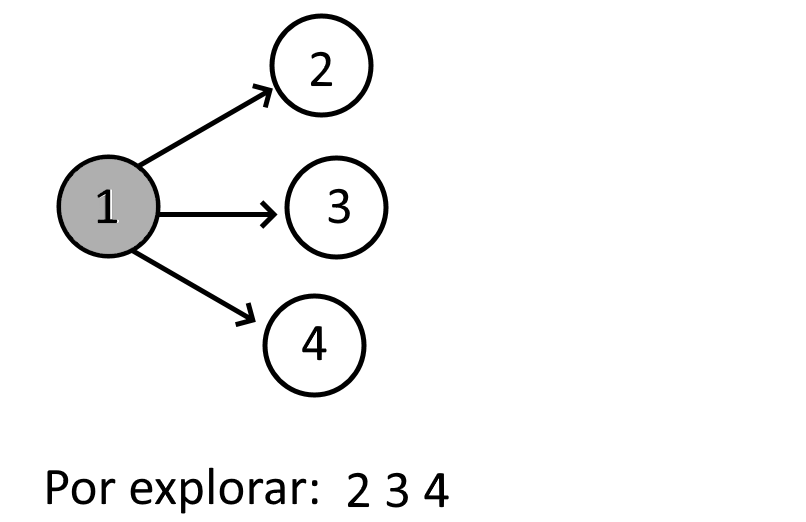
\includegraphics[scale=0.35]{bfs1}
\end{center}

Y luego para cada una de esos estados los exploramos también, es decir, expandimos las transiciones de esos estados y lo nuevo que encontremos lo ponemos en la lista de "estados por explorar". Importante: los visitamos en el orden que fueron agregados a la lista por explorar.

\begin{center}
	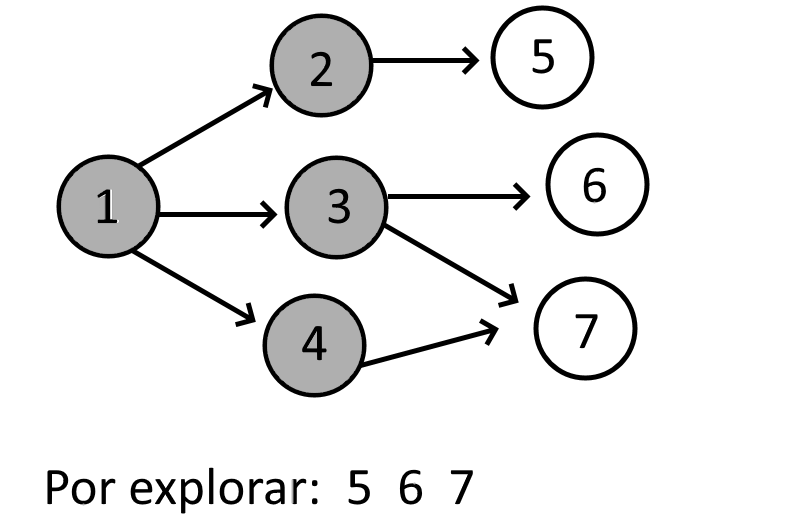
\includegraphics[scale=0.35]{bfs2}
\end{center}

De esta forma, comenzamos visitando todos los lugares alcanzables con una transición, luego dos transiciones, después tres, cuatro, cinco y  así sucesivamente.

Y precisamente, este orden en el que exploramos nos da una buena ventaja. A todo estado llegamos con la menor cantidad de transiciones posibles. Lo cual nos permite saber el mínimo número de transiciones necesarias para llegar e incluso lo podemos guardar en un arreglo o map para consultar después.

Para lograr este comportamiento, es importante ver que la lista por explorar se comporta de la siguiente forma: los estados son procesados en el mismo orden en el que entran, de forma que el primer estado en entrar a la lista es el primero en ser atendido. Este comportamiento es similar a la cola del cine, donde se atiende en el orden que llegas.

Para esto, podemos usar una estructura de datos de C++ llamada \verb|queue|, que significa cola en ingles. Si no sabes trabajar con ella, revisa el anexo en la página \pageref{queue}.

Entonces, una BFS lo que hace es:

Tener una cola de la lista por explorar llamada \verb|explorar|, un arreglo de booleanos \verb|visitado| para marcar los estados que ya han sido descubiertos por la BFS y agregaremos un arreglo de enteros \verb|no_transiciones| para guardar cuantas transiciones requerimos para llegar a cada estado.

Comenzamos agregando a la lista por explorar el estado inicial con un \verb|no_transiciones| de \(0\). Luego, mientras todavía allá estados por explorar, lo procesaremos. Lo sacaremos de la pila al ya ser explorado y agregaremos a \verb|explorar| todos los estados que no hayan sido visitados alcanzables desde el estado que estamos procesando.

En código:
\pagebreak
\begin{lstlisting}
bool visitado[];
int no_transiciones[];
void BFS(inicio) {
	queue<estados> explorar;
	cola.push(inicio);
	visitado[inicio]=true;
	no_transiciones[inicio]=0;
	while (explorar.empty()==false) {
		actual = explorar.front();
		cola.pop();
		if (actual es solucion) {
			registrar solucion actual;
			break; //opcional, si solo nos interesa una solucion
		}
		for (transiciones de actual) {
			if (!visitado[transicion]) {
				visitado[transicion]=true;
				no_transiciones[trancision]=
					no_transiciones[actual]+1;
				explorar.push(transicion);
			}
		}
	}
}
\end{lstlisting}
Como ya es de costumbre, veamos un ejemplo para entender esto.
\section*{Ejemplo 5.1}
\addcontentsline{toc}{section}{Ejemplo 5.1}
Javier tiene una calculadora un poco peculiar. Esta muestra un número \(x\) en pantalla y tiene dos botones.

\begin{plimits}
	\item El primer botón le suma \(a\) al valor de \(x\).
	\item El segundo botón le  suma \(\frac{x}{b}\) a \(x\), pero solo puede ser presionado cuando \(x\) sea un múltiplo de \(b\).
\end{plimits}

Ahora Javier se pregunta cuantas veces debe presionar un botón para que el valor \(x\) se convierta en \(y\).

\subsection*{Entrada}

La entrada constará de cuatro enteros: \(x\), \(y\), \(a\) y \(b\). El valor inicial de la calculadora, el valor deseado, y el valor de \(a\) y \(b\) para los botones.

\subsection*{Salida}
Imprime un entero que sea la cantidad de pulsaciones mínima para convertir \(x\) a \(y\). Si es imposible pasar de \(x\) a \(y\) imprime \(-1\).

\subsection*{Ejemplo}
\begin{casebox3}
	\ecase{	1 20 4 5}{6}
	{	Presiona el primer botón, ahora tienes 5.\\		
		Usa el segundo, ahora vale 6.\\
		Pulsa el primer botón, obtienes 10.\\
		Utiliza el segundo para tener 12.\\
		Usa el primer botón, obtén 16.\\
		Termina con el primero, llegamos a 20.
	}
	\ecase{	1 32 3 2}{-1}
	{	Es imposible obtener 32.
	}
\end{casebox3}

\subsection*{Límites}
\begin{plimits}
	\item \(1\leq x,y,a,b \leq 10^5\)
\end{plimits}

\section*{Solución}
Entonces, en este problema nos piden la mínima cantidad de operaciones para pasar de \(x\) al valor de \(y\).

Recordemos que la BFS es perfecta para esta situaciones, pues calcula la mínima cantidad de transiciones para pasar de un estado inicial a todos los demás, incluyendo \(y\).

Para esto haremos una BFS que use de estados el número de la calculadora y de transiciones los botones. Esta explorará todas las operaciones desde \(x\) hasta llegar a \(y\).

Esto se verá:

\pagebreak

\begin{lstlisting}
	bool visitado[100005];
	int no_transiciones[100005];
	int bfs(int x, int y, int a, int b) {
		queue<int> cola;
		cola.push(x);
		visitado[x]=true;
		no_transiciones[x]=0;		
		while (cola.empty()==false) {
			int actual=cola.front();
			cola.pop();
			if (actual==y) {
				return no_transiciones[y];
			}	
			//Primer boton
			int siguiente = actual+a;
			if (vistado[siguiente]==false){
				visitado[siguiente]=true;
				no_transiciones[siguiente]=
					no_transiciones[actual]+1;
				cola.push(siguiente);
			}
			//Segundo boton
			siguiente = actual+actual/b;
			if (actual%b == 0 && vistado[siguiente]==false){
				visitado[siguiente]=true;
				no_transiciones[siguiente]=
					no_transiciones[actual]+1;
				cola.push(siguiente);
			}
		}
		return -1;
	}
\end{lstlisting}



\section*{Complejidad}
\addcontentsline{toc}{section}{Complejidad}
La complejidad de una BFS es sencillamente de calcular. Veamos que cada estado es colocado una sola vez dentro de la cola y por lo tanto, explorado una sola vez.

Por lo tanto, cada transición también es visitada una única vez, cuando su estado correspondiente sea visitado.

Esto provoca que la complejidad de la BFS sea \(O(V+E)\), donde \(V\) es la cantidad de estados y \(E\) es el número de transiciones.

En el ejemplo 5.1, la cantidad de estados son a lo más \(y\) y a lo más tenemos dos transiciones por estado, por lo que la complejidad es \(O(V+E)=O(y+2y)=O(y)\).

\newpage

\practiceproblemsection{5}

\problemtitle Vasya encontró un dispositivo extraño. En el panel frontal hay: un botón rojo, un botón azul y una pantalla mostrando un entero positivo. 

Después de pulsar el botón rojo, el dispositivo multiplica por dos el número. Al pulsar el botón azul, el dispositivo le resta uno al número de la pantalla. 

Si en algún momento el número deja de ser positivo, el dispositivo se rompe. La pantalla puede mostrar números arbitrariamente grandes. Inicialmente se muestra el número \(n\).

Vasya quiere obtener el número \(m\) en la pantalla. ¿Cuál es la menor cantidad de pulsaciones que debe hacer para obtener este resultado?

\subsubsection*{Entrada}
La primera y única línea de la entrada tiene dos enteros distintos \(n\) y \(m\). 

\subsubsection*{Salida}
Imprime un solo número -- La mínima cantidad de veces que uno debe presionar los botones para obtener \(m\) del número \(n\).

\subsubsection*{Ejemplos}
\begin{casebox3}
	\ecase{4 6}{2}{Pulsa una vez el botón azul y luego el rojo.}
	\ecase{10 1}{9}{No necesitamos duplicar el número\\por lo que presionamos el azul nueve veces.}
\end{casebox3}

\subsubsection*{Límites}
\(1\leq n, m \leq 10^4\)

\codeforces  

\codeforceslink{520}{B}

\problembreak

\problemtitle Se te dan dos números enteros, \(n\) y \(x\). Tu puedes realizar múltiples operaciones al entero \(x\).

En cada operación que hagas consiste en: Elige un dígito \(y\) que este en la representación decimal de \(x\) al menos una vez, y remplazar \(x\) por \(x\cdot y\).

Quieres hacer que la longitud de la representación decimal de \(x\) (sin ceros a la izquierda) sea igual a \(n\). ¿Cuál es la menor cantidad de operaciones para lograr esto?

\subsubsection*{Entrada}
La única línea de la entrada contiene dos enteros \(n\) y \(x\).

\subsubsection*{Salida}
Imprime un entero -- El mínimo número de operaciones requeridas para hacer la longitud de la representación decimal de \(x\) (sin ceros a la izquierda) igual a \(n\), o \(-1\) si es imposible.

\begin{casebox3}
	\ecase{2 1}{-1}{}
	\ecase{3 2}{4}{
		1. multiplica \(x\) por \(2\), tal que \(x=2\cdot 2=4;\)\\
		2. multiplica \(x\) por \(4\), tal que \(x=4\cdot 4=16;\)\\
		3. multiplica \(x\) por \(6\), tal que \(x=16\cdot 6=96;\)\\
		4. multiplica \(x\) por \(9\), tal que \(x=96\cdot 9=864;\)\\
	}
	\ecase{13 42}{12}{}
\end{casebox3}
\subsection*{Límites}
\begin{plimits}
	\item \(2\leq n \leq 19\)
	\item \(1\leq x \leq 10^{n-1}\)
\end{plimits}
\codeforces

\codeforceslink{1681}{D}

\problembreak

\problemtitle Javier esta en un tablero de \(N\) filas y \(M\) columnas. En este tablero habrá unas celdas libres y unas celdas bloqueadas.

Él se encuentra en la casilla superior izquierda, la \((1, 1)\), y quiere llegar a la casilla \((f,c)\). La casilla donde Javier inicia siempre será libre.

Javier puede en cualquier momento, dar un paso y moverse a cualquiera de las cuatro casillas de arriba, abajo, izquierda o derecha. Siempre y cuando estas casillas existan y no estén bloqueadas. 

Determina la mínima cantidad de pasos para ir de \((1, 1)\) a \((f,c)\).

\subsubsection*{Entrada}
Dos enteros \(N\) y \(M\), el número de filas y el número de columnas del tablero.

En las siguientes \(N\) líneas recibirás \(M\) caracteres, siendo la descripción del tablero. '\#' simboliza una casilla bloqueada y '.' es una libre.

En la última línea tendrás dos enteros. \(f\) y \(c\), la fila y columna donde esta la celda a la que Javier quiere ir.

\subsubsection*{Salida}
Imprime un entero -- La mínima cantidad de pasos para ir de \((1, 1)\) a\((f, c)\). Si no se puede imprime \(-1\).

\subsubsection*{Ejemplo}

\begin{casebox3}
	\ecase{
		3 5\\
		\texttt{..\#.\#}\\
		\texttt{\#...\#}\\
		\texttt{..\#\#.}\\
		3 1
	} {		
		4
	}{
		\\
		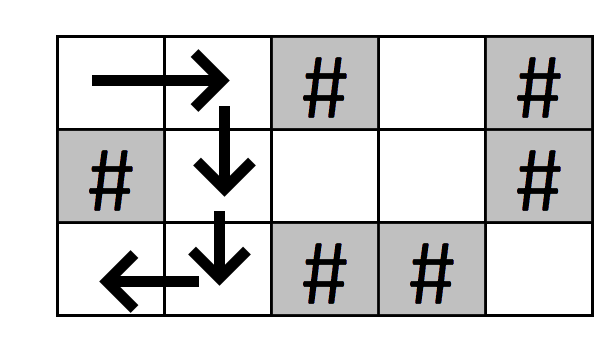
\includegraphics[scale=0.20]{caminoDFS1}
	}
	\ecase{	
		4 5\\
		\texttt{....\#}\\
		\texttt{\#...\#}\\
		\texttt{\#.\#\#.}\\
		\texttt{...\#.}\\
		3 5\\
	}{-1}{}
\end{casebox3}

\subsubsection*{Límites}
\begin{plimits}
	\item \(2\leq N, M\leq 1000\)
	\item \(1\leq f \leq N\)
	\item \(1\leq c \leq M\)
\end{plimits}

TODO \omegalink{}

\problembreak

\problemtitle Hay nueve relojes dispuestos en un arreglo de \(3 \times 3\) (véase la imagen), etiquetado con las las letras de la \(A\) a la \(I\). El objetivo d este problema  es regresar las manecillas de todos los relojes para que marquen las 12 en punto en el menor número de movimientos posibles.

\begin{center}
	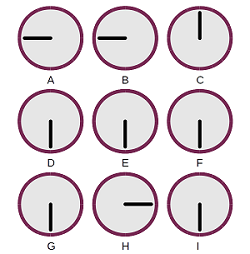
\includegraphics[scale=0.6]{relojes}
\end{center}

Hay nueve diferentes movimientos permitidos para modificar las manecillas de los relojes. Cada movimiento permitido es identificado por un número del 1 al 9. Un movimiento afecta únicamente a un determinado conjunto de relojes; cada reloj afectado mueve su manecilla 90° (grados) en sentido horario. A continuación se encuentra la descripción de los relojes afectados por los nueve movimientos:

\begin{center}
	\begin{footnotesize}
		\begin{tabular}{|ll|}
			\hline
			\thead{Movimiento} & \thead{Relojes afectados} \\
			\hline
			\makecell[c]{1} & \makecell[c]{ABDE} \\ \hline
			\makecell[c]{2} & \makecell[c]{ABC} \\   \hline
			\makecell[c]{3} & \makecell[c]{BCEF} \\  \hline
			\makecell[c]{4} & \makecell[c]{ADG} \\   \hline
			\makecell[c]{5} & \makecell[c]{BDEFH} \\  \hline
			\makecell[c]{6} & \makecell[c]{CFI} \\  \hline
			\makecell[c]{7} & \makecell[c]{DEGH} \\  \hline
			\makecell[c]{8} & \makecell[c]{GHI} \\  \hline
			\makecell[c]{9} & \makecell[c]{EFHI} \\  \hline
		\end{tabular}
	\end{footnotesize}
\end{center}

La siguiente figura muestra una posible solución para el caso presentado en la imagen de arriba, descrita por los números de movimiento 5, 8, 4 y 9. Nota que esta no es la única solución para el caso de ejemplo.


\begin{center}
	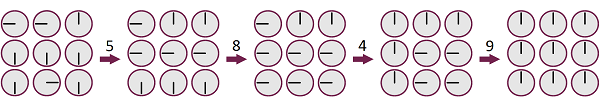
\includegraphics[scale=0.75]{relojes2}
\end{center}

\subsubsection*{Entrada}
res líneas con tres enteros cada una; cada entero representa la hora inicial de cada reloj, en el orden \(A, B, C, \ldots, H, I\). Los enteros tendrán un valor 3, 6, 9 o 12, representando la hora que marca un reloj.

\subsubsection*{Salida}
Imprime en salida estándar una sola línea con una lista de enteros separados por espacios: la secuencia de movimientos más corta que pone todos los relojes marcando las 12 en punto. En caso de que existan múltiples secuencias válidas con longitud mínima, cualquiera de ellas será aceptada.

\subsubsection*{Ejemplo}
\begin{casebox2}
	\scase{
		9 9 12\\
		6 6 6\\
		6 3 6
	}{5 8 4 9}
\end{casebox2}

Fuente: IOI 1994

\omegalink{relojes}




